\section{The Real and Complex Number Systems}
\subsection{The Naturals, Integers, and Rationals}
We begin by a review of number systems which are already familiar.

\begin{ndef}{The Natural Numbers}
    The \textbf{Naturals}, denoted by $\NN$, is the set $\set{1, 2, 3, \ldots}$.
\end{ndef}

For $x, y, \in \NN$, we have that $x + y \in \NN$ and $xy \in \NN$, so the naturals are closed under addition and multiplication. However, we note that it is not closed under subtraction; take for example $2 - 4 = -2 \notin \NN$.

\begin{ndef}{The Integers}
    The \textbf{Integers}, denoted by $\ZZ$, is the set $\set{\ldots, -3, -2, -1, 0, 1, 2, 3, \ldots}$.
\end{ndef}

The integers are closed under addition, multiplication, and subtraction. However, it is not closed under division; for example, $1/2 \notin \ZZ$. 

\begin{ndef}{The Rationals (informal)}
    The \textbf{Rationals}, denoted by $\QQ$, can be defined as $\set{\frac{m}{n}: m \in \ZZ, n \in \NN}$, where $\frac{m_1}{n_1}$ and $\frac{m_2}{n_2}$ are identified if $m_1n_2 = m_2n_1$.
\end{ndef}
We note that unlike the naturals/integers, the rationals do not have as obvious of a denumeration. This above is a good definition if we already have the same rigorous idea of what a rational number is in our mind; i.e. it works because we have a shared preconceived understanding of a rational number.

If this is not the case, it may help to define the rational numbers more rigorously/formally (even if the definition may be slightly harder to parse). As a second attempt at a definition, we can say that $\QQ$ is the set of ordered pairs $\set{(m, n): m \in \ZZ, n \in \NN}$. However, this is not quite enough as we need a notion of equivalence between two rational numbers (e.g. $(1, 2) = (2, 4)$). Hence, a complete and rigorous definition would be:

\begin{ndef}{The Rationals (formal)}
    The \textbf{Rationals}, denoted by $\QQ$, is the set $\set{(m, n): m \in \ZZ, n \in \NN}/\sim$ where $(m_1, n_1) \sim (m_2, n_2)$ if $m_1n_2 = m_2n_1$.
\end{ndef}
Under the formal definition, the rationals are a set of equivalence classes of ordered pairs, under the equivalence relation $\sim$. We note that the rationals are closed under addition, subtraction, multiplication, and division.

This formal definition might be slightly harder to parse, so it might be useful to consider an example with a similar flavour. Consider the set $X = \set{m \in \ZZ}/\sim$ such that $m_1 \sim m_2$ if $m_1 - m_2$ is divisible by 12. This is "clock arithmetic", with equivalence classes $[0], [1], [2], \ldots$ for each hour on an analog clock. A fun side note: If instead of 12 we picked a prime number, we would get a field (we will discuss what this is in a later lecture)!

Note that under this definition, $(1, 2)$ and $(2, 4)$ are different representations of the same rational number. With this definition, we would define addition such that $(m_1, n_1) + (m_2, n_2) = (m_1n_2 + m_2n_1, n_1n_2)$. Note that $(2m_1, 2n_2) + (m_2, n_2) = (2m_1n_2 + 2m_2n_1, 2n_1n_2)$ and we can identify $(m_1n_2 + m_2n_1, n_1n_2)$ with $(2m_1n_2 + 2m_2n_1, 2n_1n_2)$. If we choose different representations when we do addition, we might get a different representation in our result, but it will represent the same rational number regardless of the choice of representations we originally chose to do the addition. 

A natural question then becomes if the rationals are sufficient for doing all of real analysis. Certainly, it seems as we have a number system that is closed under all our basic arithmetic operations; but is this enough? For example, are we able to take limits just using the rationals? The answer turns out to be no (they are insufficient!) and the following example will serve as one illustration of this fact. 

\begin{example}{Incompleteness of the Rationals}{1.1a}
    (a) There exists no $p \in \QQ$ such that $p^2 = 2$.
\end{example}
We proceed via proof by contradiction. Recall in that these types of proof, we start with a certain wrong assumption, follow a correct/true line of reasoning, reach an eventual absurdity, and therefore conclude that the original assumption was mistaken. 
\begin{nproof}
    Let us then suppose for the contradiction that there exists $p = \frac{m}{n}$ with $p^2 = 2$. We then have that not both $m, n$ are even, and hence at least one is odd. Then, we have that $2 = p^2 = \frac{m^2}{n^2}$ and hence $m^2 = 2n^2$, so $m^2$ is even, implying $m$ is even. So, let us write $m = 2k$ for $k \in \ZZ$. Then, $(2k)^2 = 4k^2 = 2n^2$, and hence $2k^2 = n^2$. Therefore, $n^2$ is even and hence $n$ is even. $m$ and $n$ are therefore both even, a contradiction. We conclude that no such $p$ exists.
\end{nproof}
Why can we conclude that not both $m, n$ are even in the above proof? This is the case as if $m, n$ we both even, then we could write $m = 2m'$, $n = 2n'$ for some $m', n'$, and then $p = \frac{m}{n} = \frac{2m'}{2n'} = \frac{m'}{n'}$ which we can continue until either the numerator or denominator is odd. A natural question to consider is how to prove that this process of reducing fractions will eventually conclude. The resolution is to invoke the fundamental theorem of arithmetic, and write $m, n$ in terms of their unique prime factorization. We are then able to cancel out factors of 2 from the numerator/denominator until at least one is odd.

We note that this example leads us to conclude that the rationals have certain "holes" in them. This is concerning, as there are sequences of rational numbers that tend to $\sqrt{2}$. Conversely, its not as concerning that there is no rational number $x$ such that $x^2 = -1$, as there is no such sequence of rational numbers that is "close to" $i$ (note that both $\sqrt{2}$ and $i$ have not yet been defined, but this will come shortly).

\setcounter{rudin}{0}

\begin{example}{Incompleteness of the Rationals}{1.1b}
    (b) Let $A = \set{p \in \QQ: p > 0, p^2 < 2}$, and $B = \set{p \in \QQ: p > 0, p^2 > 2}$. Then, $\forall p \in A, \exists q \in A$ such that $p < q$, and $\forall p \in B, \exists q \in B$ such that $q < p$. 
\end{example}
\begin{figure}[htbp]
    \centering
    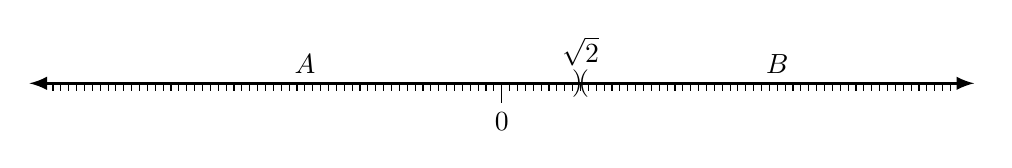
\begin{tikzpicture}
        \draw[latex-latex, very thick] (-6, 0) -- (6,0) node[anchor=south] {$\QQ$};
        \draw[] (0, 0) -- (0, -0.25) node[anchor=north] {0};
        \foreach \i in {-5.7,-5.6,...,5.7}{ 
        \draw[] (\i,0) -- (\i,-0.1);
        }
        \draw[] (1,0.1) node[anchor=south] {$\sqrt{2}$};
        \draw[] (0.96,0) node[] {$)$};
        \draw[] (1.04,0) node[] {$($};
        \draw[] (-2.5, 0) node[anchor=south] {$A$};
        \draw[] (3.5, 0) node[anchor=south] {$B$};
    \end{tikzpicture}
    \caption{Visualization of sets $A$ and $B$. We note that $\sqrt{2}$ has not been defined in our formalism yet, but from our prior mathematical intuition it would be what goes in the "hole" that the rationals have.}
    \label{<label>}
\end{figure}

For the proof of this statement, we consider playing a 2 person game. One person is $\forall$, one person is $\exists$, and we consider if one person has a winning strategy. $\forall$ goes first, and then $\exists$ goes next, having seen the choice that $\forall$ has made. Then, we check if indeed $p < q$. If $p < q$, then $\exists$ wins. If $p \not< q$, then $\forall$ wins. 

\begin{nproof}
    (b) Let $p \in A$. Then, let $q = \frac{2p + 2}{2 + p}$. Since $p \in \QQ$, it follows that $2p + 2 \in \QQ$ and $2 + p \in \QQ$ so $q \in \QQ$. Furthermore, we have that $2p + 2 > 0$ and $2 + p > 0$, so $q > 0$. We also have that:
    \[q^2 = \frac{(2p+2)^2}{(2+p)^2} = 2 + \frac{2(p^2 - 2)}{(p+2)^2} < 2\]
    Where the inequality follows from the fact that $p^2 < 2$ and hence $(p^2 - 2) < 0$. It therefore follows that $q \in A$. Finally, we have that:
    \[q = p + \frac{2-p^2}{2+p} > p\]
    so $q > p$, completing the proof of the first part of the claim. The second part is left as an exercise (we note that the same $q$ can be used).
\end{nproof}

The number $q = \frac{2p+ 2}{2 + p}$ seems to be pulled out of a hat, but actually comes from a fairly geometric picture (the secant method of approximating roots). Discussion on this topic can be found here: \texttt{https://math.stackexchange.com/questions/141774/choice-of-q-in-baby-rudins-example-1-1}.

\subsection{Ordered Sets}
Over the next couple sections, we will be discussing certain properties of sets that will give us a better understanding of the real numbers, and allow us to construct them.

\setcounter{rudin}{4}

\begin{definition}{Order}{1.5}
    An \textbf{order} $<$ on a set $S$ is a relation with the following properties:
    \begin{enumerate}
        \item For every pair $x, y \in S$, exactly one of $x < y$, $x = y$, or $y < x$ is true. 
        \item For $x, y, z \in S$, if $x < y$ and $y < z$, then $x < z$. 
    \end{enumerate}
    A point on notation; We note that $x > y$ means $y < x$, and $x \leq y$ means $x < y$ or $x = y$. 
\end{definition}

\begin{definition}{Ordered Sets}{1.6}
    An ordered set is a pair $(S, <)$. We may write just $S$ if the order can be inferred by the context.
\end{definition}
A familiar (and useful) set of examples is $S = \NN$ or $S = \ZZ$ or $S = \QQ$. For these three sets, we have that $x < y$ if $y-x$ is positive. For another example, consider the set $S$ of english words; then the order $<$ can be the dictionary/lexographic order. 

\begin{definition}{Upper \& Lower Bounds}{1.7}
    Let $S$ be an ordered set and $E \subset S$ (note that here, $E \subset S$ is a non-strict subset, and $E \subsetneq S$ is a strict subset). $E$ is \textbf{bounded above} if there exists an element $\beta \in S$ such that $\forall x \in E$, $x \leq \beta$. Any such $\beta$ is an \textbf{upper bound} of $E$. Similarly, we say that $E$ is \textbf{bounded below} if there exists an element $\alpha \in S$ such that $\forall x \in E$, $\alpha \leq x$. In this case, $\alpha$ is a \textbf{lower bound} of $E$.
\end{definition}
As an example, one can take $S = \QQ$, $E = A = \set{p \in \QQ: p > 0, p^2 > 2}$ (as in Example \ref{exam:1.1b}). Here, $E$ is bounded above, with $\beta = 2$ as one possible upper bound. to see this is the case, consider that if $p \in E$:
\[2 - p = \frac{4 - p^2}{2+p} > \frac{4-2}{2+p} > 0\]
However, if we take $S = A$, $E = A$, then $E$ is not bounded above as we saw in the example. There is no upper bound of $A$ in $A$. In general, this example reveals the subtle point that "the upper bound of a set" is ill-defined; we need to specify $E \subset S$. 

\subsection{The Least Upper Bound Property}
\begin{definition}{Least Upper Bound \& Greatest Lower Bound}{1.8}
    Let $S$ be an ordered set, and let $E \subset S$ with $E$ bounded above. If $\exists \alpha \in S$ such that:
    \begin{enumerate}
        \item $\alpha$ is an upper bound for $E$
        \item If $\gamma < \alpha$, then $\gamma$ is not an upper bound for $E$
    \end{enumerate} 
    The $\alpha$ is the \textbf{least upper bound}, or \textbf{supermum} of $E$. This can be denoted as $\alpha = \sup(E)$. Analogously, the \textbf{greatest lower bound}, or \textbf{infimum} of E (denoted $\alpha = \inf(E)$) is an element $\alpha \in S$ (if it exists) such that:
    \begin{enumerate}
        \item $\alpha$ is a lower bound for $E$
        \item If $\gamma > \alpha$, then $\gamma$ is not an upper bound of $E$. 
    \end{enumerate}
\end{definition}

\begin{ntheorem}{Uniqueness of supremum/infimum}
    If the supremum/infimum of $E \subset S$ exist, they are unique.
\end{ntheorem}
\begin{nproof}
        Let $E \subset S$. Suppose that there exist $\alpha_1, \alpha_2$ such that $\alpha_1 = \sup(E)$ and $\alpha_2 = \sup(E)$. If $\alpha_1 < \alpha_2$, as $\alpha_1$ is an upper bound of $E$, this contradicts the fact that $\alpha_2$ is the least upper bound of $E$. We reach an identical contradiction if $\alpha_2 < \alpha_1$. Therefore we conclude that $\alpha_1 = \alpha_2$ and the supremum of $E$ is unique (if it exists). The proof for the infimum is analogous. 
\end{nproof}

\begin{ntheorem}{Equivalence of maximum and supremum}
    If $E \subset S$ has a maximum element $\alpha$ (that is, an element such that $x < \alpha$ for all $x \in E$) then $\alpha = \sup(E)$. Similarly, if $E$ has a minimum element $\alpha$, then $\alpha = \inf(E)$. The proof is left as an exercise. 
\end{ntheorem}

\begin{comment}
\begin{nproof}
    Let $E \subset S$ and $\alpha = \max(E)$. By definition $\alpha$ is an upper bound of $E$, and if $x < \alpha$ for some $x \in E$ then $x$ is not an upper bound of $E$ as it is not greater than $\alpha \in E$. The claim follows (with an identical proof for the minimum).
\end{nproof}
\end{comment}

\begin{example}{}{1.9}
    \begin{enumerate}
        \item Consider again the sets $A, B \subset \QQ$ from example \ref{exam:1.1b}. $A$ is bounded above by any element in $B$, and the upper bounds of $A$ are exactly the elements of $B$. Since $B$ has no smallest member, $A$ does not have a least upper bound in $\QQ$.
        \item Let $E_1, E_2 \subset \QQ$ such that $E_1 = \set{r: \QQ, r < 0}$ and $E_2 = \set{r: \QQ, r \leq 0}$. Then $\sup(E_1) = \sup(E_2) = 0$. Note that this example shows that the supremum can either be contained or not contained in the set; $0 \notin E_1$ but $0 \in E_2$. 
        \item Let $E \subset \QQ$ such that $E = \set{\frac{1}{n}: n \in \NN}$. Then $\sup(E) = 1$ and $\inf(E) = 0$. This is proven below. 
    \end{enumerate}
\end{example}
\begin{nproof}
    $\sup(E) = 1$ immediately follows from the equivalence of the maximum and supremum as proven above. To see that $\inf(E) = 0$, first note that $0$ is a lower bound for $E$ as all of the elements of $E$ are positive. To see that it is the lower bound, take any $x > 0$. Then, we have that for any $n > \frac{1}{x}$, $\frac{1}{n} < x$ and hence $x$ is not an upper bound of $E$. This proves the claim.
\end{nproof}

\begin{definition}{The LUB/GUB Property}{1.10}
    An ordered set $S$ has the \textbf{least upper bound property} if for every $E \subset S$, if $E \neq \emptyset$ and $E$ is bounded above, then $E$ has a least upper bound (that is, $\sup(E)$ exists in $S$). Similarly, an ordered set $S$ has the \textbf{greatest lower bound property} if for every $E \subset S$, if $E \neq \emptyset$ and $E$ is bounded below, then $E$ has a greatest lower bound.
\end{definition}
We will show in the next theorem that these properties are actually equivalent; before then, we briefly consider two examples.
\begin{nexample}{$\ZZ$ and $\QQ$}
    $\ZZ$ has the least upper bound property, while $\QQ$ does not. 
\end{nexample}
\begin{nproof}
    For the first claim, consider any nonempty $E \subset \ZZ$ that is bounded above. Choose any $x \in E$. Since $\ZZ$ is bounded above, there exist finitely many elements that are greater than $x$. Take the maximum of these finitely many elements. This maximum is also the maximum of $E$, so it is the supremum of $E$. Therefore $\ZZ$ has the LUB property as claimed.
    
    The second claim immediately follows from Example \ref{exam:1.9}(a). 
\end{nproof}

\begin{theorem}{Equivalence of LUB/GUB properties}{1.11}
    Let $S$ be an ordered set. Then $S$ has the LUB property if and only if it has the GUB property. 
\end{theorem}
\begin{nproof}
    $\boxed{\implies}$ Let $S$ be an ordered set with the LUB property. Let $E \subset S$ with $E \neq \emptyset$, with $E$ bounded below. Let $L = \set{x \in S: x\text{ is a lower bound of $E$.}}$. $L \neq \emptyset$ as $E$ is bounded below (and hence has at least one lower bound). If $y \in E$, then $y$ is an upper bound for $L$. Since $E$ is nonempty, $L$ is therefore bounded above. Since $S$ has the LUB property, then $\sup(L)$ must exist. Let us call this $\alpha$. Then, $\alpha \leq x\ \forall x \in E$ (as if $\gamma < \alpha$, then $\gamma$ is not an upper bound of $L$ and hence $\gamma \neq E$). Hence, $\alpha$ is a lower bound for $E$ and hence $\alpha \in L$. Since $\alpha = \sup(L)$ and $\alpha$ is an upper bound for $L$, we have that $\alpha \geq \gamma\ \forall \gamma \in L$. Thus, $\alpha = \inf(E)$. 

    $\boxed{\impliedby}$ Left as an exercise. 
\end{nproof}

\subsection{Fields and Ordered Fields}
\begin{definition}{Fields}{1.12}
    A field $F$ is a set with two binary operations, $+$ and $\cdot$ (addition and multiplication) such that the following axioms are satisfied:
    \begin{enumerate}[start=1, label={(A\arabic*):}]
    \item If $x, y \in F$, then $x + y \in F$. (Closure under addition)
    \item $x + y = y + x$ for all $x, y \in F$. (Commutativity of addition)
    \item $(x+y) + z = x + (y + z)$ for all $x, y, z \in F$. (Associativity of addition)
    \item $\exists 0 \in F$ such that $\forall x \in F$, $0 + x = x$. (Additive identity)
    \item $\forall x \in F$, $\exists y$ such that $x + y = 0$. We can denote $y = -x$. (Additive inverse)
    \end{enumerate}
    \begin{enumerate}[start=1, label={(M\arabic*):}]
        \item If $x, y \in F$, then $x\cdot y\in F$. (Closure under multiplication)
        \item $x \cdot y = y \cdot x$ for all $x, y \in F$.
        \item $(x\cdot y)\cdot z = x \cdot (y \cdot z)$ for all $x, y, z \in F$. (Associativity under multiplication)
        \item $\exists 1 \in F$ such that $1 \neq 0$ and $\forall x \in F$, $1 \cdot x = x$. (Multiplicative identity)
        \item $\forall x \in F$, exists $y \in F$ such that $x \cdot y = 1$. We can denote $y = \frac{1}{x}$. (Multiplicative inverse)
    \end{enumerate}
    (D): $x \cdot (y + z) = x \cdot y + x \cdot z$, $\forall x, y, z \in F$. (Distributive law)
\end{definition}
Note that A3/M3 show that $x + y + z$ and $x\cdot y\cdot z$ are well defined in a mathematical sense; however, associativity may not hold for computers that do math with finite precision! 
\begin{ntheorem}{Uniqueness of Identities and Inverses}
    The additive/multiplicative identities given by (A4)/(M4) and the additive/multiplicative inverses given by (A5)/(M5) are unique. 
\end{ntheorem}
\begin{nproof}
    Let $F$ be an ordered field. Suppose that there exist $0_1, 0_2 \in F$ such that $0_1 + x= x$ and $0_2 + x = x$ for all $x \in F$. We then have that:
    \begin{align*}
        0_1 + 0_2 &= 0_1 + 0_2
        \\ 0_1 + 0_2 &= 0_2 + 0_1 & \text{(A2)}
        \\ 0_2 &= 0_1 & \text{(Property of additive identity)}
    \end{align*}
    Which shows that the additive identity is unique. The remaining proofs are left as an exercise.
\end{nproof}
In Rudin, some easy (and familiar) consequences of the field axioms can be found in Propositions 1.14-1.16. Instead of repeating those here, we will 